\documentclass[]{scrreprt}

\usepackage[utf8]{inputenc}	

\renewcommand{\baselinestretch}{1.5} 

\usepackage{graphicx}
\usepackage{float}


% Title Page
\title{Projeto de Inovação com Algoritmos Genéticos}
\author{José Geraldo de Carvalho Pereira}


\begin{document}

\maketitle

%\begin{abstract}
%\end{abstract}

\chapter{Introdução}
\section{Autômatos celulares}

Os autômatos celulares foram inventados na década de 40 por John von Neumann baseando-se em sugestões de seu colega, o matemático Stanislaw Ulan \cite{citeulike:12886945}. Autômatos celulares são modelos matemáticos para representar sistemas complexos e consistem num conjunto de células discretas espacialmente que apresentam um estado dentre um
conjunto finito de estados possíveis. Os autômatos celulares evoluem paralelamente, ou seja, o estado de cada célula evolui de maneira síncrona em passos discretos de tempo e de acordo com regras simples e determinísticas gerando uma complexidade a partir do efeito cooperativo de elementos simples – as regras e as células – tratando-se portanto de uma complexidade emergente, que surge globalmente no sistema a partir de regras simples, locais e determinísticas \cite{Wolfram19841}.

Autômatos celulares tem sido utilizados em diversos campos de pesquisa 
como por exemplo na modelagem de sistemas: (1) biológicos, desde eventos intracelulares, como redes de interação proteicas, até estudo de populações; (2) químicos, na modelagem cinética de sistemas moleculares e no crescimento de cristais; (3) físicos, para o estudos sistemas dinâmicos, desde a interação entre partículas até o agrupamento de galáxias \cite{Ganguly03asurvey}. 

\begin{figure}
	\label{ca}
	\includegraphics[width=1\linewidth]{ca_final}
	\caption{Exemplo de um autômato celular elementar. Este é o tipo de autômato celular mais simples, pois é unidimensional, possui apenas dois estados (0 ou 1) e possui vizinhança 1 (uma célula a esquerda e uma a direita). O autômato inicia com um linha de células ($t_{0}$) e evolui através da aplicação de uma regra de transição que irá determinar o estado de cada uma das células na geração seguinte ($t_{1}$). Este processo ocorre iterativamente produzindo, muitas vezes, uma complexidade global que emerge da aplicação da regra local.}
\end{figure}

\section{Autômatos celulares aplicados a predição da estrutura secundária proteica}

Neste trabalho buscamos utilizar autômatos celulares para predizer a estrutura secundária de proteínas (Figura \ref{ca_ss}). Assim como os autômatos celulares elementares (Figura \ref{ca}), os autômatos celulares que planejamos são unidimensionais e possuem vizinhança um, ou seja, cada célula evolui de acordo com o seu estado atual e o estados de seu vizinho a esquerda e a direita. Entretanto, esse autômato celular não possui apenas dois estados (0 ou 1) como os elementares e portanto, cada regra não é composta apenas de 8 elementos, mas de 13824 elementos (Equação \ref{eq_rules}).

\begin{eqnarray*}\label{eq_rules}
nElementos & = & (nAA + nSS + n\#)^3\\
		   & = & (20 + 3 + 1)^3\\
           & = & 13824
\end{eqnarray*}

Onde $nAA$ é o número de aminoácidos (20), $nSS$ é o número de elementos da estrura secundária (3 = hélice, fita, alça) e $n\#$ é o sinal de início/término da cadeia polipeptídica. O expoente 3 é resultado do número de células que determinam o estado seguinte, nesse caso, o estado da própria célula e os estados dos vizinhos, um a esquerda e um a direita. 

Cada um desses 13824 elementos da regra de transição podem evoluir pra quatro estados possíveis. Três deles representam elementos de estrutura secundária e um deles representa um estado indefinido o qual indica que a célula assumirá um estado igual ao seu estado inicial (estado em $t_{0}$).

Desses 13824 elementos, 576 deles possuem o sinal de início/término $\#$ na célula central. Esses elementos evoluem sempre para o estado $\#$ para conservar o sinal de início/término da cadeia polipeptídica. Outros 23 elementos possuem ambos os vizinhos com o sinal de início/término $\#$ e permanecerão constantemente no estado inicial $t_{0}$. Assim, somente os 13225 elementos restantes poderão assumir um dos quatro estados possíveis mencionados anteriormente. Nosso problema resume-se, portanto, em encontrar a melhor combinação desses 13225 elementos capaz de predizer a estrutura secundária proteica. 

\begin{figure}
	\label{ca_ss}
	\includegraphics{ca-ss_final}
	\caption{Esquema de um autômato celular para a predição de estruturas secundárias. A regra de transição do autômato é composta de 13824 elementos. O estado inicial do autômato ($t_{0}$) é formado pela sequência de aminoácidos da proteína. O estado $\#$ indica o início ou o fim da cadeia polipeptídica e pode ser utilizado para concatenar múltiplas proteínas, funcionando como uma barreira de influência entre elas. O estado final do autômato celular $t_{n}$, onde $n$ é um número finito, é a estrutura secundária predita e sua similaridade com a estrutura secundária atribuída pode ser considerada uma medida do fitness da regra de transição.}
\end{figure}

\section{Algoritmo genético na busca da regra de transição do autômato celular}

A busca de uma regra de transição capaz de reproduzir um padrão desejado no autômato celular é conhecido como o "problema inverso". Como mencionado anteriormente, neste trabalho buscamos encontrar a melhor combinação para 13225 elementos da regra de transição, sendo que cada um desses elementos podem assumir um entre quatro estados possíveis. Logo, o espaço de regras é igual a $4^{13225}$ regras. Esse enorme espaço de regras torna essencial a utilização de um método de busca como por exemplo, algoritmos genéticos (Figura \ref{ca_ga}).




\begin{figure}
	\label{ca_ga}
	\includegraphics{ca_ga_final}
	\caption{Representação da utilização de um algoritmo genético na busca por uma regra de transição capaz de predizer estrututuras secundárias proteicas. Os cromossomos possuem 13225 genes, ou variáveis, que podem assumir quatro estados distintos. Cada indivíduo apresenta uma combinação desses estados. Essa combinação corresponde a uma regra de transição de um autômato celular que irá evoluir por um número definido de passos. A comparação do resultado dessa evolução com a estrutura secundária atribuída ("real") fornece uma medida do fitness da regra. Utilizando-se um algoritmo genético competente esperasse que ocorra uma convergência para a regra com maior fitness, ou seja, a que melhor prediz a estrutura secundária da proteína.}
\end{figure}

\chapter{Análise do problema}

\section{Tamanho da população}
O primeiro passo no design de algoritmos genéticos competentes é o cálculo para estimar o tamanho da população. O tamanho da população $N$ pode ser estimado usando a equação (\ref{eqn}) desenvolvida por Harik e colaboradores \cite{Harik:1999:GRP:1326811.1326813}, a qual considera dois fatores que influenciam na convergência para uma solução ótima: (1) o suprimento inicial de building blocks (BBs) e a seleção dos melhores BBs em detrimento de seus competidores.

A equação (\ref{eqn}) é baseada em um modelo de \textit{random walk} que representa o suprimento e a competição entre BBs como o Problema da Ruína do Jogador.

\begin{equation}\label{eqn}
N \ge -2^{k-1}\ln(\alpha)\frac{\sigma_{bb}\sqrt{\pi(m-1)}}{d}
\end{equation}

Onde $k$ é o tamanho do BB, $\alpha$ é a probabilidade de falha, $\sigma_{bb}$ é o desvio padrão do fitness dos BBs, $d$ é a diferença entre o melhor e o segundo melhor BB e $m$ representa o número máximo de BBs. O termo $\sigma_{bb}\sqrt{\pi(m-1)}$ representa a interferência do ruído na competição entre BBs \cite{WRCR:WRCR8771}.

Para, por exemplo, assegurar a convergência para uma solução próxima a ótima com uma probabilidade maior que 95\%, o $\alpha$  deve ser menor que 5\%.

Em nosso problema temos 13225 variáveis, ou genes, cada uma com 4 estados possíveis ($S^{ss}$) ao invés de estados binários. Como ocorre esse aumento no número de estados, nossa equação para estimar o $N$ é modificada para:

\begin{equation}\label{eqn2}
N \ge -4^{k-1}\ln(\alpha)\frac{\sigma_{bb}\sqrt{\pi(m-1)}}{d}
\end{equation}

No entanto, como nosso problema tem $k=1$ devido a independência entre os elementos das regras de transição dos autômatos celulares, o resultado da equação não é alterado pelo número de estados $S^{ss}$.

Para estimar os valores de $\sigma_{bb}$ e $d$ foram gerados 500000 indivíduos. Essa amostra foi utilizada para calcularmos o fitness médio e o desvio padrão do fitness para cada um dos 4 estados possíveis dos 13225 genes. A diferença entre o maior fitness médio dentre os 52900 calculados e o fitness médio de seu melhor competidor, ou seja, no mesmo BB, foi utilizado para estimarmos $d$ (Tabela \ref{tab_fit}) e resultou em $d=0,001972661$. O valor de $\sigma_{bb}$ foi definido como sendo a média dos 52900 $\sigma$ calculados de cada BB e resultou em $\sigma_{bb}=0.0241745599487$.

Parâmetros:
\begin{itemize}
	\item $k=1$
	\item $m=13225$
	\item $\sigma_{bb}=0.0241745599487$
	\item $d=0,001972661$
\end{itemize}

\begin{table}[h]
	\begin{tabular}{c c c c c}
		\#BB & alça & hélice & fita & indefinido \\ \hline
		0 &	0.23449416747 & 0.23431394377 & 0.234057267599 & 0.234641266667 \\ 
		1 &	0.234400559059 & 0.23418784333 & 0.234336782416 & 	0.234589721927 \\
		2 &	0.234334660854 & 0.235053426835	 & 0.23364863406 &	0.234490579159 \\
		3 &	0.234793579586 &	0.233538815916 &	0.234522613316 &	0.234683748762 \\
		4 &	0.235535591828 &	0.233493969724 &	0.234588961624 &	0.233911300129 \\
		... & ... &... &... &...\\
	\end{tabular}   
	\caption{Fitness médio dos estados por BBs. O fitness médio foi calculado para cada um dos 13225 BBs. Neste segmento da tabela utilizado como exemplo, o BB com maior fitness médio é o BB 4 com estado igual a alça (0.235535591828). Logo, seu maior competidor é o estado fita, também do BB 4 (0.234588961624), pois BBs em outros locais - outros números - não são competidores. Considerando esse exemplo, $d$ seria igual a $0.235535591828-0.234588961624$, logo $d=0,00094663$.}
	\label{tab_fit}
\end{table}
 
 Com os parâmetros calculados e considerando $\alpha=0.01$, conseguimos estimar que $N\ge11502,9$ (Figura \ref{fig_n}).


\begin{figure}
	\label{fig_n}
	\includegraphics{fig1}
	\caption{O gráfico demonstra o tamanho da população estimado pela probabilidade de convergência $P_{c}$, onde $P_{c}=1-\alpha$.}
\end{figure}

\section{Complexidade computacional}

Após a estimação do tamanho da população, podemos analisar a complexidade do GA. A complexidade é medida como o número de funções necessárias para atingir a solução ótima e pode ser calculada como o número de gerações, ou tempo de convergência, multiplicado pelo tamanho da população. 

O tempo de convergência é afetado pela taxa relativa com que os genes convergem. Por exemplo, quando todos os genes são igualmente importantes para a solução e a convergência ocorre uniformemente, o tempo de convergência é  uma função de $O(\sqrt{l})$, onde $l$ é o tamanho da string de genes. Quando a importância de cada gene varia, a convergência ocorre sequencialmente e consequentemente, o tempo de convergência é uma função de $O(l)$. Esses dois casos representam o limite inferior e superior da complexidade do tempo de convergência.

Assumindo uma seleção por torneio, temos que o tempo de convergência para todas as strings, assumindo uma convergência sequencial dos genes (\emph{domino convergence}) é \cite{Thierens:1994:CMG:645822.670524,Thierens98dominoconvergence}:

\begin{equation}\label{eqt}
t = 2l
\end{equation}

Assim, podemos estimar um tempo de convergência colocando um limite superior calculado pela equação \ref{eqt}. Considerando $l=2*13225$, pois cada gene precisa de dois bits para ser representado, temos que o tempo de convergência máximo será de 52900 gerações. Entretanto, como todas as variáveis são importantes para o autômato, acreditamos que a convergência poderá ocorrer uniformemente e portanto a partir de 162 gerações ($t=\sqrt{l}$).

Considerando o tempo de convergência máximo estimado $t=52900$ e uma população estimada $N=11502$ conseguimos estimar que poderão ser necessárias aproximadamente 600 milhões de avaliações.

\section{Deriva genética}

A deriva genética ocorre em uma população quando a mutação e o crossover fazem os genes flutuarem e convergirem para um solução não ótima na ausência de uma pressão seletiva.

O número esperado de gerações para os genes convergirem na ausência de pressão seletiva para uma população inicial de strings binárias geradas randomicamente com proporções iguais de 0s e 1s é estimado como \cite{Thierens98dominoconvergence}:

\begin{equation}\label{eqtderiv}
t_{deriv} = 1.4N
\end{equation}

O que resulta em $t_{deriv}=18515$.

A equação \ref{eqtderiv} mostra que o tempo de convergência devido a deriva genética é uma função linear do tamanho da população. Para assegurar que uma ocorra uma convergência para um ótimo ao invés de uma convergência por deriva genética podemos satisfazer a condição.

\begin{equation}\label{eqttd}
t < t_{deriv} 
\end{equation}

No nosso caso, o tempo de convergência máximo obtido pela equação \ref{eqt} foi $t=52900$. Consequentemente, deveríamos aumentar $N$ para aproximadamente 37785, o que elevaria para quase 2 bilhões o número de avaliações necessária no pior caso.

\chapter{Conclusão}

O design de algoritmos genéticos competentes reduz o tempo gasto na busca por parâmetros que resultem em soluções ótimas e fornece estimativas do tamanho do problema. No nosso caso, conseguimos estimar diversos parâmetros, por exemplo:

\begin{itemize}
\item No pior caso, onde teríamos uma convergência sequencial dos genes, o número de gerações necessárias seria aproximadamente 50000 e necessitaríamos de uma população aproximada de 40000 indivíduos para evitar uma convergência por deriva genética. Isso resultaria em quase 2 bilhões de avaliações. Considerando o tempo de cada avaliação igual a 0.5s/CPU, teríamos o total necessário de 280 mil horas/CPU, ou seja, 30 anos/CPU, o que tornaria o problema inviável.

\item No melhor caso teríamos um convergência uniforme dos genes e portanto, o número de gerações necessárias seria de aproximadamente 162. Como o número de gerações seria menor que o tempo de convergência por deriva genética, poderíamos manter $N=11502$. Isso resultaria em um número de avaliações necessárias menor que 2 milhões, ou 280 horas/CPU. Assim, o melhor caso tem uma ordem de grandeza 1000 vezes menor que o pior caso, necessitando apenas de 12 dias/CPU.
\end{itemize}

Os elementos das regras de transição dos autômatos celulares são independentes entre si e todos são necessários para a evolução do autômato celular. Tais características sugerem que a convergência deverá ocorrer de maneira uniforme, e consequentemente teremos uma convergência mais próxima ao "melhor caso" analisado acima. 

\bibliographystyle{apalike}
\bibliography{biblio}

\end{document}          
